\documentclass[11pt, a4paper]{article}

\usepackage{graphicx}
\usepackage[a4paper,top=3cm,bottom=2cm,left=2cm,right=2cm,marginparwidth=1.75cm]{geometry}
\usepackage[english]{babel}
\usepackage[utf8x]{inputenc}
\usepackage{subfig}
\usepackage{float}
\usepackage{amsmath}
\usepackage{amssymb}
\usepackage{mhchem}
\usepackage{hyperref}
\usepackage{tikz}
\usepackage{cancel}
\usepackage{bm}

\graphicspath{ {./images} }
\newcommand*{\qed}{\hfill\ensuremath{\quad\square}}%
\newcommand*{\rad}{\ensuremath{\,\text{rad}}}
\newcommand*{\R}{\ensuremath{\mathbb{R}}}
\newcommand*{\C}{\ensuremath{\mathbb{C}}}
\renewcommand*{\Re}{\operatorname{Re}}
\renewcommand*{\Im}{\operatorname{Im}}
\renewcommand*{\epsilon}{\varepsilon}
\renewcommand*{\phi}{\varphi}
\renewcommand*{\d}{\,\text{d}}

\DeclareRobustCommand{\uvec}[1]{{%
  \ifcat\relax\noexpand#1%
    % it should be a Greek letter
    \bm{\hat{#1}}%
  \else
    \ifcsname uvec#1\endcsname
      \csname uvec#1\endcsname
    \else
      \bm{\hat{\mathbf{#1}}}%
     \fi
   \fi
}}

\makeatletter
\renewcommand*\env@matrix[1][*\c@MaxMatrixCols c]{%
  \hskip -\arraycolsep
  \let\@ifnextchar\new@ifnextchar
  \array{#1}}
\makeatother

\newtheorem{theorem}{Theorem}
\numberwithin{equation}{section}
\numberwithin{figure}{section}

%------------------------------------------------
%Templates for images and figures
% \begin{figure}[h]
%   \centering
%   \subfloat[caption 1]{{
\includegraphics[width=30mm]{images/placeholder.png}}}%
%   \qquad
%   \subfloat[caption 2]{{
\includegraphics[width=30mm]{images/placeholder.png}}}%
%   \caption{Description}
% \end{figure}

% \begin{figure}[h]
%   \centerline{
\includegraphics[width=50mm]{images/placeholder.png}}
%   \caption{Description}
% \end{figure}

%Template for a simple table 
%\begin{table}[h]
%   \caption{Description} %title of the table
%   \centering % centering table
%   \begin{tabular}{l rr} % creating three columns
%     \hline\hline %inserting double-line
%     & & \\ [0.5ex] % Insert half line vertical spacing
%     \hline % inserts single-line
%     & & \\ 
%     & & \\
%     & & \\
%     & & \\
%   \hline % inserts single-line
%   \end{tabular}
%   \label{tab:hresult}
% \end{table}
%-----------------------------------------------

\begin{document}
\setcounter{section}{4}
\section{Power series}

\subsection{The Geometric series as a power series}
Recall that the geometric series was given as:
\begin{equation}
    \sum_{n=0}^\infty x^n = 1 + x + x^2 + x^2 + \cdots
\end{equation}
The series converges for $-1 < x < 1$, in which case the series is given as:
\begin{equation}
    \sum_{n=0}^\infty x^n = \frac{1}{1-x}
\end{equation}
The terms of the polynomial when thought of as power series will start approximating the graph of $\frac{1}{1 -x}$ closer and closer for larger choices of the partial sum $n$. This is visualised in the figure below.
\begin{figure}[H]
  \centerline{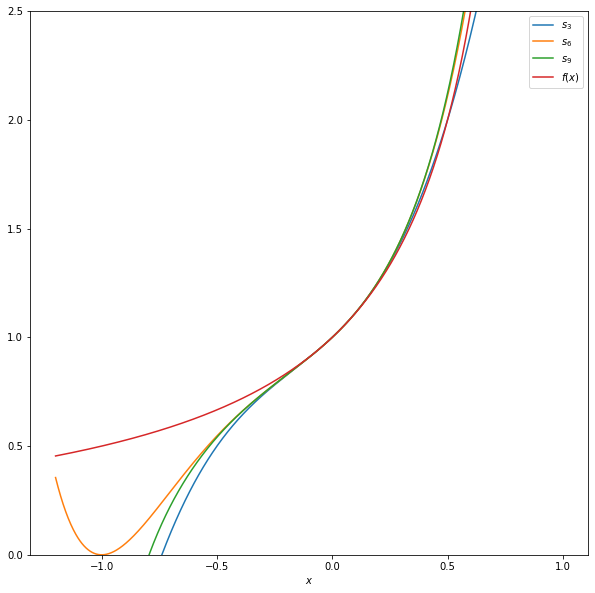
\includegraphics[width=80mm]{images/Approximating_f.png}}
  \caption{The terms of the polynomial $s_n = \sum_{n=0}^n x^n$ approximating the graph of $f(x) = \frac{1}{1-x}$ closer and closer for larger choices of $n$.}
\end{figure}
We already know from studying the geometric series in an earlier lecture that the limit only exists when:
\begin{equation}
    \lim_{n\to\infty} s_n = \frac{1}{1-x} \quad \text{if} \quad -1 < x < 1
\end{equation}
Thus we are lead to the conclusion that if $f(x) = \sum_{n=0}^\infty c_n(x-a)^n$, then $f(x)\approx s_n$ where $s_n =c + c_1(x-a) + c_2(x-a)^2 + \cdots + c_n(x-a)^n$.\\
\\ \underline{Example:}  
\begin{equation*}
    \frac{1}{5-x} = \frac{1}{1 - (x-4)} = \sum_{n=0}^{\infty} (x-4)^n
\end{equation*}
The condition for the polynomial to exists is:
\begin{gather*}
    -1 < (x-4) < 1\\
    3 < x < 5
\end{gather*}
Thus:
\begin{equation*}
    \frac{1}{5-x} \approx s_6 = \sum_{n=0}^6 (x-4)^i
\end{equation*}


\subsection{Defining a power series}
Let $x \in \R$. A power series is then given as:
\begin{equation}
    \sum_{n=0}^\infty c_n(x-a)^n = c_0 + c_1(x-a) + c_2(x-a)^2 + \cdots
\end{equation}
The $c_n$ terms are called the coefficients and $a$ is the center of the polynomial. Every power series will satisfy 1 of the following 3 conditions:
\begin{enumerate}
    \item The series converges (absolutely) for all $x\in\R$
    \item The series converges only for $x=a$
    \item There exists a number $R > 0$ such that the series converges (absolutely) if $|x-a| < R$ and diverges for $|x-a|>R$.
\end{enumerate}
In case 3 the number $R$ is referred to as the radius of convergence. The best way to determine $R$ is by using the root or ratio test.
\\
\\ \underline{Example:}
\begin{equation*}
    \sum_{n=0}^\infty \frac{x^n}{n!} \quad \text{Let} \quad a_n = \frac{x^n}{n!}
\end{equation*}
Applying the ratio test we find that:
\begin{equation*}
    \lim_{n\to\infty} \left| \frac{a_{n+1}}{a_n} \right| = \lim_{n\to\infty} \left| \frac{x^{n+1}}{(n+1)!} \,\Big/\, \frac{x^n}{n!} \right| = \lim_{n\to\infty} \frac{|x|}{n+1} = 0 \quad \text{for all}\; x\in\R
\end{equation*}
Thus the series converges absolutely for all $x\in\R$.
\begin{equation*}
    \sum_{n=0}^\infty \frac{(x-1)^{2n}}{n2^n} \quad \text{Let} \quad a_n = \frac{(x-1)^{2n}}{n2^n}
\end{equation*}
Applying the ratio test here we find:
\begin{align*}
    \lim_{n\to\infty} \left| \frac{a_{n+1}}{a_n} \right| &= \lim_{n\to\infty} \left| \frac{(x-1)^{2(n+1)}}{(n+1)2^{n+1}} \,\Big/\, \frac{(x-1)^{2n}}{n2^n} \right|\\  
    &= \lim_{n\to\infty} \frac{(x-1)^2}{2}\cdot\frac{n}{n+1} = \frac{(x-1)^2}{2}
\end{align*}
Thus this series converges absolutely for $(x-1)^2 < 2$. This means the series diverges for $x = 1\pm \sqrt{2}$. This give the convergence interval $(1-\sqrt{2}, 1 + \sqrt{2})$.


\subsection{Integrating and differentiating power series}
One big advantage of power series is the fact that all terms are polynomial terms. We like those because they are easy to integrate and differentiate. If $p(x)$ is some $n$-th degree polynomial we get:
\begin{align}
  p(x) &= c_0 + c_1(x-a) + c_2(x-a)^2 + \cdots + c_n(x-a)^n\\
  \frac{\d p(x)}{\d x} &= c_1 + 2c_2(x-a) + 3c_3(x-a)^3 + \cdots + nc_n(x-a)^{n-1}\\
  \int p(x)\d x &= C + c_0(x-a) + \frac{1}{2}c_1(x-a)^2 + \cdots + \frac{1}{n-1}c_n (x-a)^{n+1}
\end{align}
Applying this to the power series we can write the derrivative $s'(x)$ of some power series $s(x) \sum_{n=0}^\infty x_n(x-a)^n$ and the integral $S(x)$ of this power series as:
\begin{align}
  s'(x) &= \frac{\d s(x)}{\d x} = \sum_{n=0}^\infty nc_n(x-a)^{n-1}\\
  S(x) &= \int s(x)\d x = C + \sum_{n=0}^\infty \frac{c_n}{n+1}(x-a)^{n+1}
\end{align} 

\end{document}